\chapter{Realizace} \label{realizace}
% Popis implementace/realizace se zaměřením na nestandardní části řešení.
% A tady budu řešit jednotlivé Cisco příkazy - jak jsem na to přicházel, postupné problémy, moje implementace a odchylky.

% \begin{itemize}
%  \item směrování prijmiEthernetove()
%  \item wrapper pro routovací tabulku
%  \item překlad adres
%  \item příkaz Uloz
%  \item SAXHandler
%  \item CiscoParserPrikazu
%  \item Cisco příkazy
%     \begin{itemize}
%      \item Parsery
%      \item ???
%     \end{itemize}
% \end{itemize}

Téméř všechny části systému obsahují tzv. debugovací mód, který vypisuje extra informace, co se právě děje nebo přidává další vlastnost vhodnou pro ladění.

\section{Parser Cisco}
Po návrhu a implementaci jádra systému se moje úsilí přesunulo k parseru příkazů pro Cisco. 
% Metoda \verb|zpracujRadek()| je klíčová, protože to je právě ona, kdo rozhoduje, komu bude předáno řízení programu. 

\subsection{Cisco IOS}
Cisco IOS je operační systém, který se nachází na drtivé většině směrovačů firmy Cisco Systems. IOS obsahuje pouze ovládání přes příkazový řádek - CLI\footnote{Command Line Interface}. Pro mě je to spíše výhodou, protože je to mnohem jednodušší na implementaci ve srovnání s \uv{klikacím} GUI\footnote{Graphical User Interface}. IOS má implementováno tzv. zkracování příkazů, které zefektivňuje práci s celým systémem. Celé to funguje tak, že když uživatelův začátek příkazu lze doplnit na jedinečný příkaz (samotné doplnění přes klávesu \verb|TAB|), tak to takový příkaz hned zavolá. Například příkaz \verb|sh run| lze jednoznačně doplnit na \verb|show running-config|, ale kratší \verb|sh ru| už ne:
\begin{verbatim}
Router#sh ru?
rudpv1  running-config
\end{verbatim} 

IOS tvoří několik stavů, např.:
\begin{itemize}
 \item uživatelský mód
 \item privilegovaný mód
 \item konfigurační mód - zde se nastavují volby, které ovlivní celý systém
 \item konfigurace rozhraní - konfigurace jednoho určitého rozhraní
\end{itemize}

\begin{figure}[h]
\begin{center}
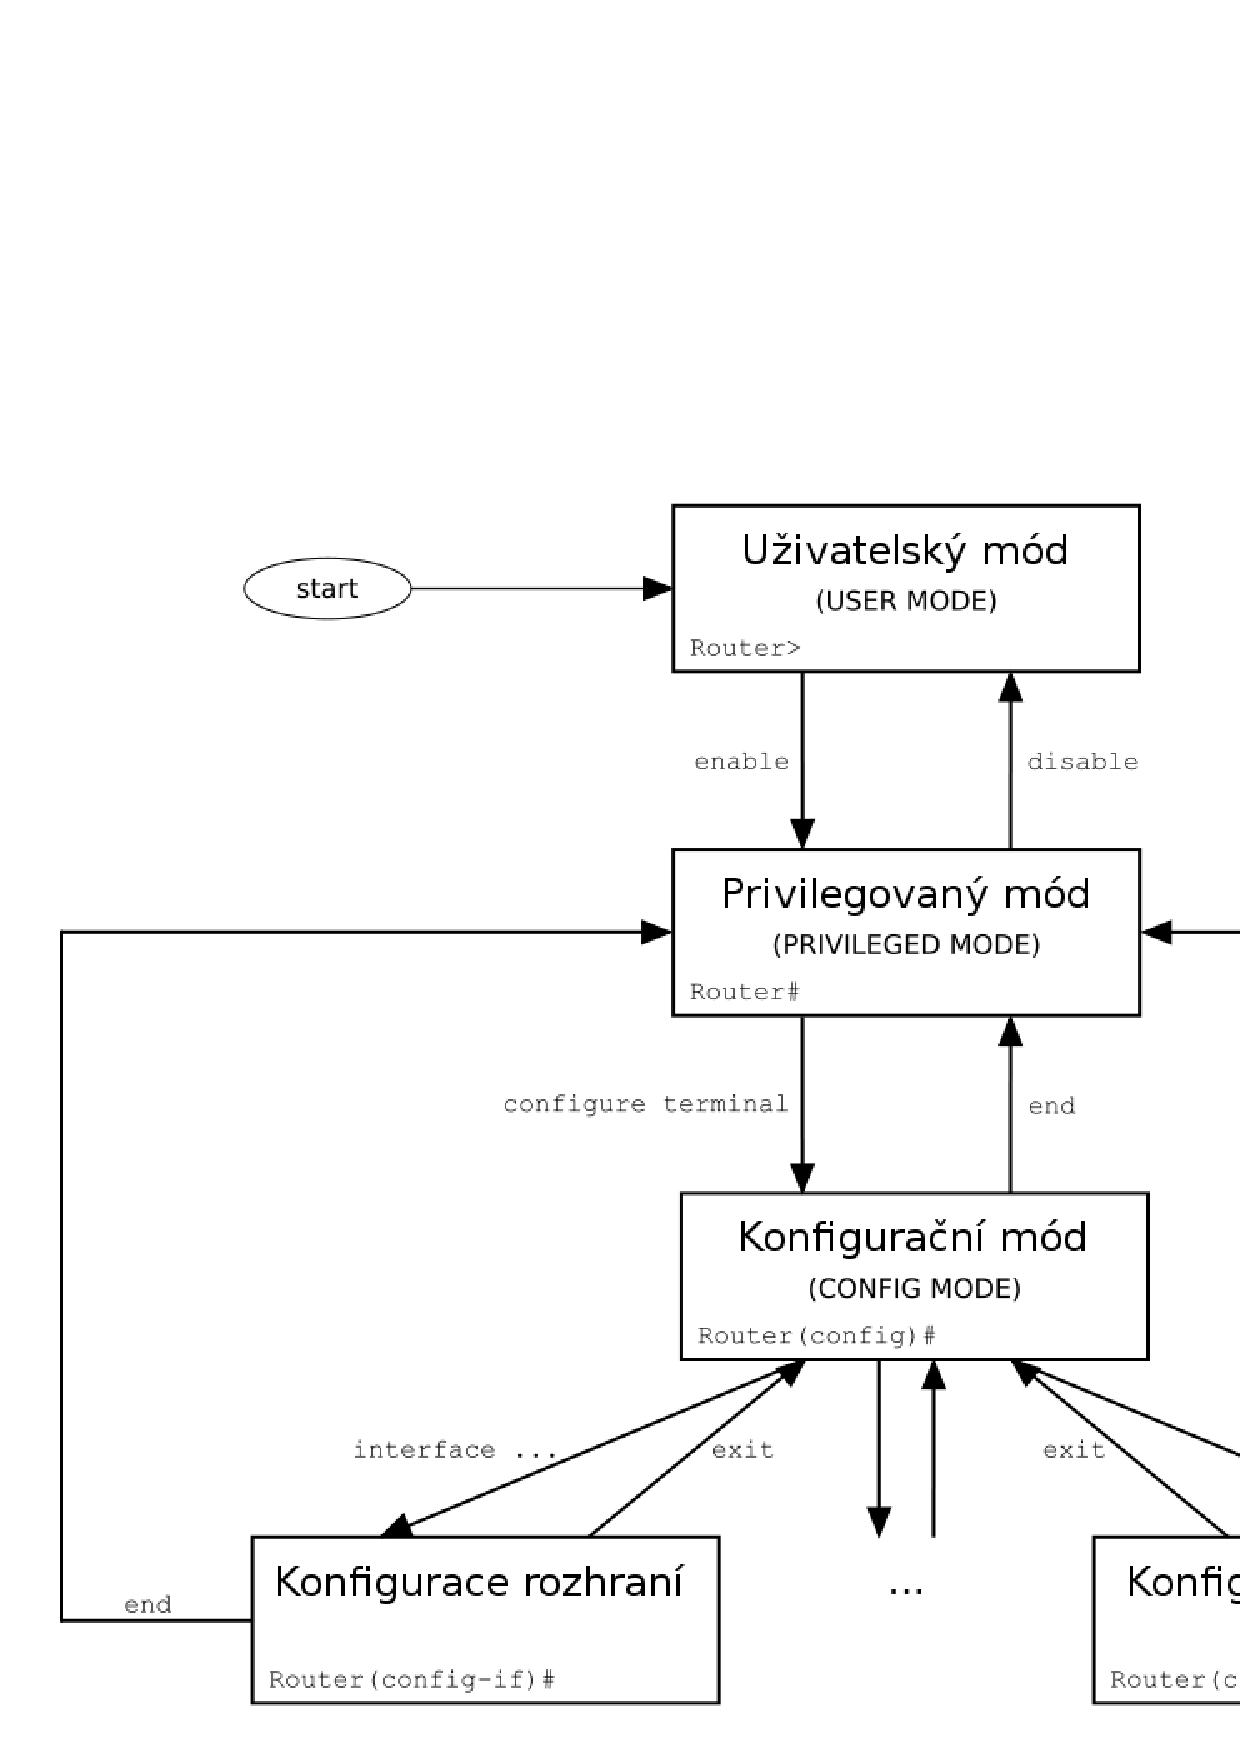
\includegraphics[width=13cm]{figures/ios.png}
\caption{Přehled základních módů Cisco IOS \cite{wiki:ios}}
\label{fig:ios}
\end{center}
\end{figure}

Na obrázku \ref{fig:ios} jsou zobrazeny důležité stavy IOS a přechody mezi nimi. 

\subsubsection{Uživatelský mód}
Uživatelský mód (USER MODE) je výchozí (startovací) mód. Tento mód je značně limitovaný a dovoluje použití čistě read-only příkazů (tj. takových, které nezmění konfiguraci). Přesto má tento mód svoje opodstatnění, dovoluje např. výpis směrovací tabulky \verb|show ip route| či příkazy \verb|ping| nebo \verb|traceroute|. Do privilegovaného režimu se lze přepnout příkazem \verb|enable|.

\subsubsection{Privilegovaný mód}
Privilegovaný mód (PRIVILEGED MODE) nebo také \uv{administrátorský} mód je podobný linuxovému \verb|root| účtu. Tento mód je výchozím bodem pro vstup do ostatních módů. Pro návrat zpět do uživatelského režimu existuje příkaz \verb|disable|. Příkaz \verb|configure| způsobí přepnutí do dalšího konfiguračního módu. Tento stav umožnuje vypsat veškeré informace o aktuální konfiguraci systému, např.:
\begin{itemize}
 \item \verb|show running-config| - shrnutí aktuální konfigurace
 \item \verb|show ip route| - výpis směrovací tabulky
 \item \verb|show ip nat translations| - výpis dynamických záznamů v NAT tabulce
\end{itemize}
Není důvod, proč by v tomto stavu nefungovaly příkazy \verb|ping| a \verb|traceroute|.

\subsubsection{Konfigurační mód}
Konfigurační mód (CONFIG MODE) je jeden z nejdůležitějších, protože umožňuje konfiguraci směrovacích záznamů (\verb|ip route ..|), přístupových seznamů pro potřeby překladu adres (\verb|ip nat inside source ..|), pooly IP adres (\verb|ip nat pool ..|) a výběr rozhraní pro přechod do stavu konfigurace rozhraní (\verb|interface ..|).

\subsubsection{Konfigurace rozhraní}
V tomto módu lze nastavovat IP adresy na aktuálně vybrané rozhraní, nastavovat příznaky pro veřejné a soukromé rozhraní pro NAT (\verb|nat inside|, \verb|nat outside|) nebo také zapínat či vypínat rozhraní. Pro přechod ze všech konfiguračních módů do privilegovaného stačí napsat příkaz \verb|end| nebo jen stisknout klávesovou zkratku \verb|Ctrl+Z|.


\subsection{Implementace Cisco IOS}
Cisco IOS obsahuje desítky příkazů z nichž každý může mít až stovky variací. Proto jsem implementoval pouze úzkou část příkazů, která je potřebná pro splnění zadání této práce. Nejdůležitější funkcí parseru je rozpoznávání zkrácených příkazů. Na skutečném Ciscu se opravdu procházejí všechny možnosti, které mohou v daném stavu nastat, a podle nich probíhá vyhodnocování. V mé implementaci ale mám pouze část příkazů, takže jsem to musel vyřešit jiným způsobem. Pro každé slovo (část příkazu) si \verb|CiscoParserPrikazu| drží počet písmen, který je potřeba k jednoznačnému určení příkazu. Tato čísla jsem \uv{naměřil} na školních ciscách v březnu 2010. Zajímavé je, že už o 2 měsíce později jsem objevil drobné změny. Čísla se mohou měnit s různými verzemi Cisco IOS. To bych ale neviděl jako zásádní problém. Většina studentů (alespoň dle mé zkušenosti) stejně píše celé příkazy a zkrácené verze nepoužívá.

Vyhodnocování příkazů zajišťuje metoda \verb|kontrola(command, cmd)|. Parametr \verb|command| je celý příkaz, na který by se to mohlo eventuelně doplnit, a \verb|cmd| je příkaz poslaný od uživatele. Nejdříve se zjistí počet znaků, který je potřeba pro jednoznačné doplnění na příkaz \verb|command|. Po té se zkontroluje požadovaný počet znaků a také jestli zkrácený příkaz odpovídá doplněnému. A jak to vypadá v kódu:

\begin{verbatim}
if (cmd.length() >= i && command.startsWith(cmd)) {
    // lze doplnit na jeden jedinecny prikaz
    return true;
}
if (command.startsWith(cmd)) {
    // vypsat amiguous command
    nepokracovat = true;
}
\end{verbatim}

Jednotlivé příkazy Cisco IOS jsou implementovány v samostatných třídách. Třída \\\verb|CiscoParserPrikazu| tedy zajišťuje přechody mezi stavy (módy) a \uv{nahazování} rozhraní. Přepnutí stavu rozhraní je natolik triviální, že se by se nevyplatilo mít pro to zvláštní třídu. 

\paragraph{}
Ladící mód zjednodušuje testování parseru a přidává tyto funkce:
\begin{itemize}
 \item klávesa \verb|Enter| funguje jako přechod z uživatelského do privilegovaného módu
 \item použití příkazů z jiných módů v privilegovaném módu - navíc např. \verb| ip route|, \\\verb|ip nat pool inside|, \verb|access-list|, ..
 \item extra výpis dynamických záznamů v natovací tabulce
 \item výpis \verb|show running-config| je pro přehlednost zkrácen
 \item možnost testování routovací tabulky přes linuxový příkaz \verb|route|
 \item používání linuxového příkazu \verb|ifconfig|
\end{itemize}
Použití těchto věcí je vhodné spíše pro ladění programu do budoucna než pro běh v \uv{ostrém} provozu.

Má implementace Cisco IOS má navíc pár příkazů, které jsou potřeba pro ovládání systému. Jak už jsem se zmiňoval v kapitole \ref{kap:podobnost} je zde navíc \verb|help| a \verb|help_en| pro výpis nápovědy. Příkaz \verb|kill| přijde vhod, když uživatel chce ihned vypnout aplikaci a nechce projít přes několik stavů příkazem \verb|exit|. Další servisní příkaz je \verb|save| nebo také \verb|uloz|, který zapíše aktuální konfiguraci všech počítačů do konfiguračního souboru. Dále lze využít velmi jednoduchý příkaz \verb|?| (otazník), který vypíše seznam dostupných příkazů v aktuálním stavu.

% \lstinline{System.out.println("Tady je text")}

\section{Načítání ze souboru}

\section{Ukládání do souboru}

\section{Směrování}\label{prijmiEthernetove}

\section{Wrapper směrovací tabulky}

\section{Překlad adres}


